\documentclass{scrartcl}


\usepackage[utf8]{inputenc}
\usepackage{geometry}
\usepackage{graphicx}


\geometry{
    paper=a4paper,
    left=16.5mm,
    right=16.5mm,
    top=19.48mm,
    bottom=19.48mm
}

\pagenumbering{gobble}


\newcommand{\card}[1]{%
    \IfFileExists{../images/#1.png}{%
        \includegraphics[width=59mm, height=86mm]{../images/#1.png}%
    }{%
        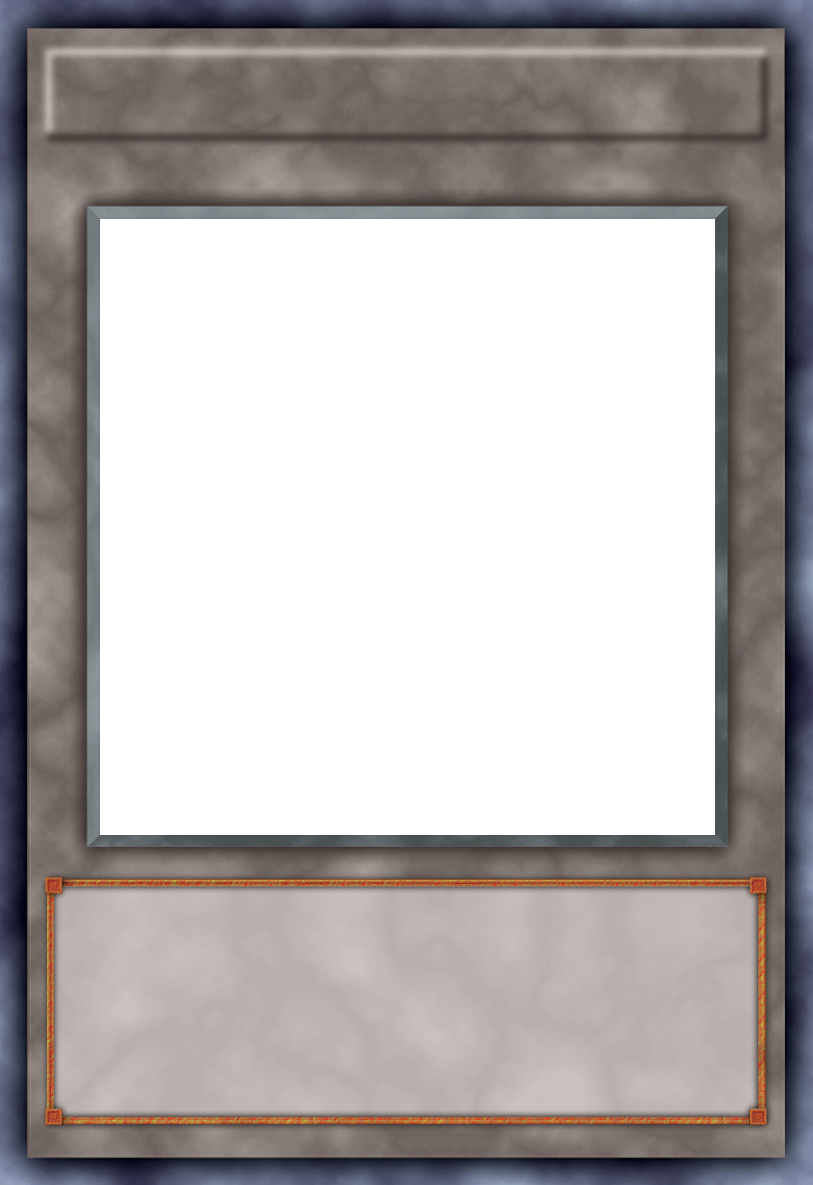
\includegraphics[width=59mm, height=86mm]{card-not-found.png}%
        \llap{%
            \raisebox{78mm}{%
                \resizebox{49mm}{\height}{%
                    \textsc{\detokenize{#1}}%
                }%
            }%
            \hspace{5mm}%
        }%
    }%
}

\begin{document}

    \noindent
    \input{cards}

\end{document}


% the contents of cards.tex are generated by a script and should look something like this:

% \card{Mystical_Space_Typhoon}%
% \card{Solemn_Strike}%
% \card{Solemn_Strike}%
% \\[-0.34mm]
% \card{Solemn_Strike}%
% \card{Solemn_Strike}%
% \card{Effect_Veiler}%
% \\[-0.34mm]
% \card{Effect_Veiler}%
% \card{Effect_Veiler}%
% \card{Mystical_Space_Typhoon}%
% \\[-0.34mm]
% \card{Mystical_Space_Typhoon}%
% \card{Mystical_Space_Typhoon}%
% \card{Mystical_Space_Typhoon}%
% \\[-0.34mm]
% \card{Mystical_Space_Typhoon}%
% \card{Solemn_Strike}%
% \card{Solemn_Strike}%
% \\[-0.34mm]
% \card{Effect_Veiler}%
